\documentclass[a4paper, 11pt]{article}
\usepackage[utf8]{inputenc}
\usepackage{graphicx}

\newcommand{\ilc}[1]{\texttt{#1}} % inline-code

\title{Report: Unidirectional NCM}
\author{Andreas Bauer, Lion Steger}
\date{April 2021}

\begin{document}
	\maketitle
	
	\section{Objective}
	Before the start of our project, the NCM module featured bidirectional sessions only.
	Our goal was to replace the current session handling with unidirectional session handling.
	\\
	For this change we needed to consider the following components: session management (\ilc{session.c}) and generation management (\ilc{generation.c}), as well as the \ilc{rlnc} library.
	\\
	Session and generation management were to be re-engineered from scratch.
	The rewrite included designing a revised acknowledgment scheme to fit the unidirectional coding scheme.
	
	\section{Outcome}
	We managed to implement the objective described above without any major drawbacks and without changes to the \ilc{librlnc} library. This was possible since we could just ignore the reverse direction of the coding matrix by setting its dimension to zero.
	We included unit tests to check for correct functionality and used the ping command for a real-world scenario test case. Furthermore, we employed a range of CI and memory tools to verify our work.
	We rewrote the session and generation management functionality in \ilc{session.c} and \ilc{generation.c} and adapted the code of \ilc{ncm.c}. This included changing some structures like headers and adding some structures for internal use, like metadata structs. A more detailed description of our new stuctures and algorithms can be found in our presentation (\ilc{docs/presentation}).
	
	\newpage
	
	\section{Transmission Performance}
	Since we could not find any flaws in functionality, we wanted to check if there are any disadvantages of our implementation regarding performance.
	First, we conducted a ping test.
	\begin{figure}[h]
		\centering
		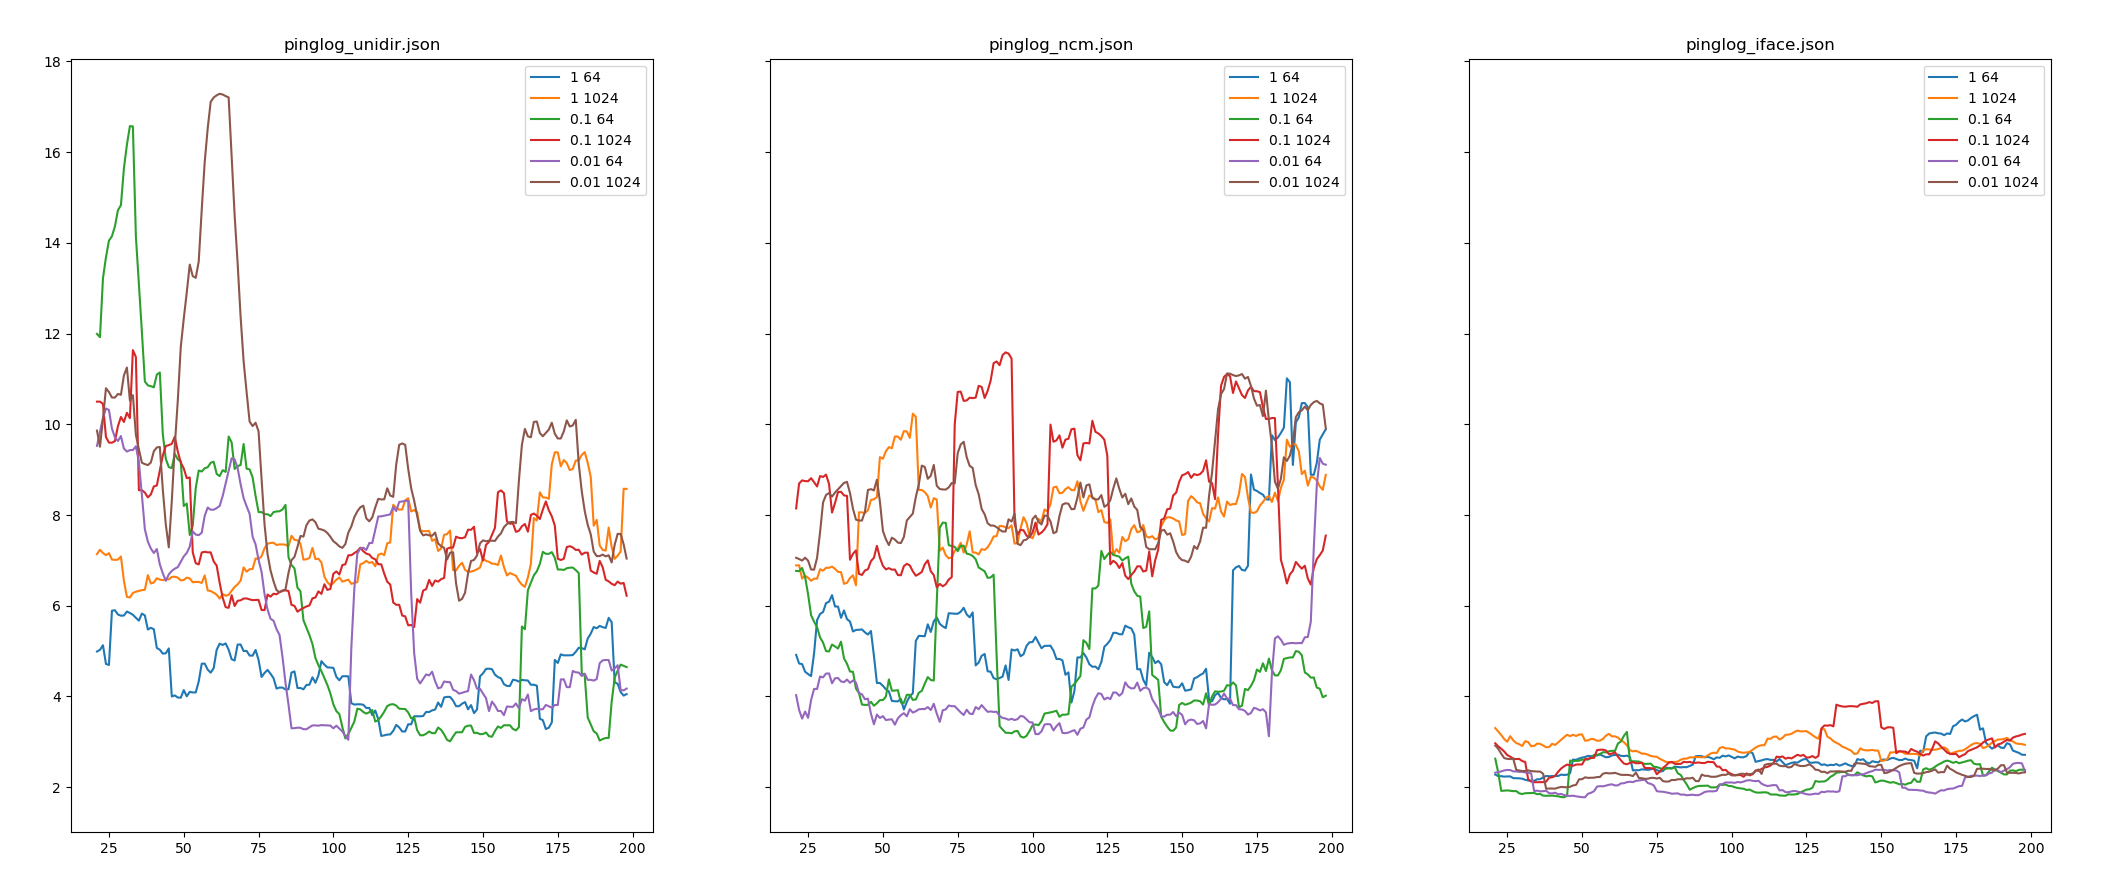
\includegraphics[scale=0.2]{ping_plot}
		\label{ping plot}
	\end{figure}
	We tested pings with different intervals (per second) and different amounts of data (bytes), comparing our implementation (unidir) with the original one (ncm) and the normal interface without network coding (iface). The y-axis shows the time response time in milliseconds, averaged over a moving windows of 20 iterations, while the iterations are shown on the x axis.
	
	Furthermore, we wanted to analyze the peak throughput rate of our implementation with \ilc{iperf3} (unidirectional test, TCP for unthrottled tests, UDP for throttled). We did encounter a problem with our generation advancement scheme because we can experience graceful exits on extreme loads. This is similar to the original implementation, which has no throughput after a certain point of time. Therefore we throttled the throughput for one test and introduced a variant with a lower chance of exiting for another test.
	\begin{figure}[h]
		\centering
		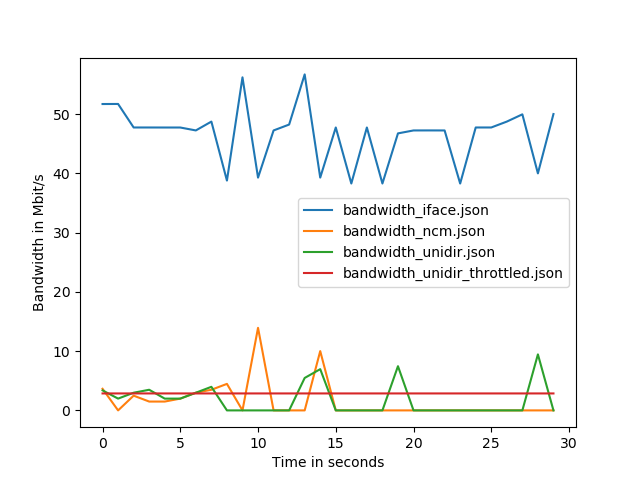
\includegraphics[scale=0.4]{bandwidth_plot}
		\label{ping plot}
	\end{figure}

	Both tests show that our implementation has a similar performance to the original one and is able to achieve stable transmission rates.
\end{document}